\documentclass{article}
\usepackage{graphicx}
\usepackage{geometry}
\usepackage[hidelinks]{hyperref}
\usepackage{rotating}
% \usepackage{biblatex}

\geometry{
    a4paper,
    total={170mm,257mm},
    left=20mm,
    top=20mm,
}

% \bibliography{references}

\title{Single-cyclist crash classification guide}
\author{
  Benjam\'in Gonz\'alez\\
  \small{\href{mailto:b.gonzaleztoledo@tudelft.nl}{B.GonzalezToledo@tudelft.nl}}
  }
\date{\today}

\begin{document}

\maketitle

%\begin{sidewaysfigure}
%    \centering
%    \includegraphics[width = \textwidth]{class-mindmap-v3.png}
%    \caption{Flowchart of bicycle crash classification.}
%    \label{fig: flowchart}
%\end{sidewaysfigure}

\begin{figure}[h]
    \centering
    
\includegraphics[scale=1.0]{bike-dof.png}
    \caption{Rotation axes of the bicycle.}
    \label{fig: bike-dof}
\end{figure}

\begin{figure}[h]
    \centering
    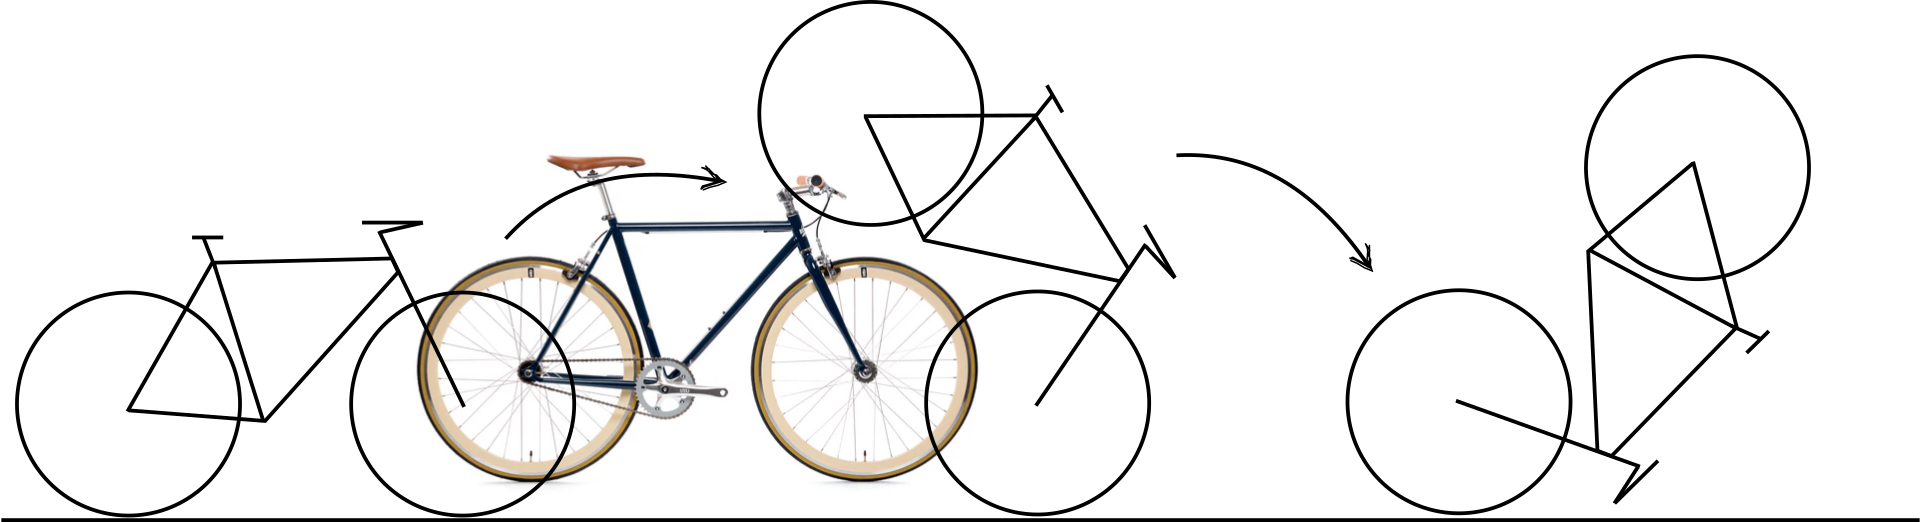
\includegraphics[width=\linewidth]{pitch-over.png}
    \caption{Simple diagram of pitch-over motion.}
    \label{fig: pitchover}
\end{figure}

\begin{figure}[h]
    \centering
    \includegraphics[width=\linewidth]{roll-over.png}
    \caption{Simple diagram of roll-over motion.}
    \label{fig: rollover}
\end{figure}

\begin{figure}[h]
    \centering
    \includegraphics[width=\linewidth]{high-side-draw.jpg}
    \caption{Hand draw of a high-side crash.}
    \label{fig: highside}
\end{figure}




\section{Introduction}

This document aims to guide you to understand the proposed classification of single-cyclist crashes and label the samples sent to you.

\subsection{What is a single-cyclist crash?}

A single-cyclist crash is an event where the normal riding of the bicycle is disrupted and ends in a crash with no other road users involved.
%
Essentially, in this document will be assumed that a crash occurs when, during a manoeuvre, one or more excitations modify the state of the system in an unexpected way.
%
This excitation is the beginning of the `critical scenario', where we find the mechanisms that produce the crash.
%
Finally, the crash itself can be characterised by the motion of the bicycle and/or the rider in the outcome of the event.



\section{Bicycle dynamics-oriented classification}

The proposed workflow to classify the crash according to the observed characteristics is composed by four layers: manoeuvre, excitation of the system, mechanisms, and motion.
%
This multi-layer approach allows to classify the crash events with different depth levels according to the available information.
%


\subsection{Manoeuvre}

The first layer consists on the manoeuvre that the rider is executing at the moment of entering to the critical scenario.
%
Here, we understand straight-running as the action of riding a straight path, maintaining balance through minor steering adjustments and no major variations on the states of the system.
%
Longitudinal acceleration manoeuvres refer to braking and acceleration, both performed by the user.
%
Steady and planned cornering refers to the situation where the rider is performing a controlled turning with a defined trajectory.
%
Low speed makes reference mainly to start and stop riding, where users require major steerign control inputs to maintain the bicycle in upright position.
%
Unplanned turning or avoidance manoeuvre is when the rider executes a sudden evasive turn or abrupt brake application to avoid an obstacle.
%
Stunting refers to any action that is not explicitly required for normal riding, such as riding with one hand, no hands, or standing on the pedals, which limits the control of the rider on the bicycle.


\subsection{Excitation of the system}

For this research, the bicycle is assumed as an interface between the human and the environment.
%
Therefore, the bicycle is subjected to forces from the environment and from human control.
%
Additionally, the bicycle itself is a dynamic system which can present excitations in its motion, which are referred as intrinsic excitations.


\begin{itemize}
    \item \textbf{External excitations (Ext):} Mechanical forces that result from the interaction of the human-bicycle system with the environment.
    \item \textbf{Intrisic excitations (Int):} Behaviour of the system due to its dynamical properties.
        %
        Its associated crash scenario is the excitation of a natural frequency of the system, creating an unstable and/or uncontrollable vehicle.
        %
        Possible mechanical failures on the bicycle also fit in this category.
    \item \textbf{Rider forces (Rid):} This makes reference to the control inputs from the human to the vehicle.
\end{itemize}



\subsection{Mechanisms of crash}

Here we detail mechanisms that make possible bicycle riding, however, in the analysis of crashes, we delve into the failure of these mechanisms.

\begin{itemize}
    \item \textbf{Modes of vibration:} Bicycles are studied as dynamical systems composed, among others, by rear and front frame connected by a rotating joint that creates the steering.
        %
        When these models are linearised, stability analyses show two particularly dangerous oscillatory modes of vibration when unstable: weave and wobble.
        %
        Being the former a combination of roll and yaw angle, while the latter a high-frequency steering oscillation.
    \item \textbf{Rider-bicycle joint:} Events where the rider is unexpectedly disengaged from the bicycle, loosing the connection to the control interfaces.
    \item \textbf{Balance control:} This refers to the lateral control of the bicycle through the steering input.
    \item \textbf{Load transfer:} This referst to the longitudinal load transfer as a result of longitudinal acceleration.
        %
        This can be caused by wrong control inputs on brake use, front collisions, objects stuck on the front wheel, etc.
    \item \textbf{Tyre friction:} Forces acting in the tyre-ground interface, principally grip and normal.
        %
        Its failure is understood as a loss of traction.
    \item \textbf{Contact forces:} All forces that interact with the human-bicycle system as contact inputs (e.g. collisions, wheel interactions different from friction)
    \item \textbf{Aerodynamic forces:} Aerodynamic forces which are studied as a resultant in the centre of pressure of the system.
\end{itemize}


\section{Important notes}

\subsection{Control interfaces}

\begin{itemize}
    \item \textbf{Handlebar:} Through the handlebar the rider exerts steering torque to control the lateral balance of the bicycle.
    \item \textbf{Pedals:} In the pedals, the rider applies force to create the propulsion of the bicycle.
        %
        This interface is subjected to large forces when the system is in longitudinal acceleration.
    \item \textbf{Brakes:} To reduce the longitudinal speed of the system, the rider controls the brakes through handles.
        %
        If the control input is not precise, the system experiences excessive braking force, over its load transfer limits.
\end{itemize}


\subsection{Motion of the bicycle}

This is related to the main motion of the rear frame of the bicycle while the crash is occuring.
%
Due to the dynamics of the bicycle, and following the common simplification to its analysis, we find two main motions related to the degrees of freedom: pitch-over and roll-over.
%
Additionally, the roll-over motion includes its own sub-classification according to the direction of rotation with respect to the initial motion.
% 
Please visit \url{https://youtube.com/shorts/_etyqSpH10c?feature=shared} to watch an example of a crash where the roll angle is negative with respect to the intended turn.
%
This is particularly challenging to represent in a normal drawing so the visual explanation is on the make, on Figure \ref{fig: highside} it is possible to see the main schematics of this kind of crash.

\begin{itemize}
    \item \textbf{Pitch-over (P):} The main characteristic of this motion is one of the wheels lifting from the ground, following a trajectory that finishes with the front wheel behind the rear wheel.
    \item \textbf{High-side (H):} Characterised for a sudden deceleration of the wheel while in lateral motion, which leads to a violent negative roll rate with respect to the direction of the initial motion.
    \item \textbf{Low-side (L):} The human-bicycle system follows an excessive roll rate in the same direction as at the beginning.
\end{itemize}

Please note that in Pitch-over and High-side motions, the rider is abruptly ejected from the bicycle.




\section{Example}

Let's do an example using the following video \url{https://youtube.com/shorts/VZibdrdhdgM?feature=shared}.

First, it is observed that the main motion of the bicycle in the crash is related to roll angle, in the same direction as at the beginning of the motion.
%
Therefore, this corresponds to the category low-side (L).


Second, from visual inspection, it is possible to conclude that the saturation limit of tyre grip was reached, causing a loss of grip during the turn.


Third, there are no visible wrong rider control inputs, which leads to a external force mechanism.
%
Additionally, it is no visible contact or aerodynamics forces playing a major role.


Finally, the classification of this crash would be \textbf{L-Tyre-Ext}, low side slide.


\section{Closing words}

This classification aims to provide a wide coverage of bicycle crashes, taking into account factors, mechanisms and common motions.
%
However, it is still possible that with the available information, the event does not fit properly in the available options.
%
For this reason, this work allows to classify crashes with a combination of different layers.



\begin{thebibliography}{9}

    \bibitem{Jac04} Elin K. Jacob (2004):  Classification and Categorization: A Difference that makes a Difference. Graduate School of Library and Information Science. University of Illinois at Urbana-Champaign. \url{http://hdl.handle.net/2142/1686}

    \bibitem{Moo12} Moore, Jason (2012): Human Control of a Bicycle. Doctoral thesis, University of California Davis.


\end{thebibliography}


\end{document}
